\documentclass[a4paper,11pt]{article}
\usepackage[utf8]{inputenc}
\usepackage{amsmath}
\usepackage{amsfonts}
\usepackage{amssymb}
\usepackage{graphicx}
\usepackage{braket}

\numberwithin{equation}{section}
\renewcommand\thesubsection{\alph{subsection}}
\newcommand{\bvp}[1]{\mathbf{#1}'}
\newcommand{\bv}[1]{\mathbf{#1}}
\newcommand{\ez}{\epsilon_0}
\newcommand{\eo}{\epsilon_1}
\newcommand{\lrp}[1]{\left({#1}\right)}
\newcommand{\lrb}[1]{\left\{{#1}\right\}}


%opening
\title{Computational Biophysics HW7}
\author{Vince Baker}

\begin{document}

\maketitle

\section{Q1}
To find the acceptance probabilities for deleting a particle we need to find the ratio of probabilities $\rho(n)/\rho(m)$ with state n having one less particle.
In the grand canonical ensemble, removing a particle i changes the energy both by removing the energy contribution $V(r_i)$ and also by changing $N\rightarrow N-1$.
The grand partition function will still factor out, so our general expression is:
\begin{align}
 \frac{\rho(n)}{\rho(m)} &= \frac{e^{-\beta(V_{N-1}-\mu (N-1)}V^{N-1}}{e^{-\beta(V_{N}-\mu N)}V^{N}}\frac{N!}{(N-1)!} = \frac{N}{V}e^{-\beta(V(r_i)+\mu)}
\end{align}
If this ratio is greater than 1, we accept the transition from m to n (deleting a particle) with probability 1, and accept the transition from n to m (creating a particle) 
with probahility $\frac{N}{V}e^{-\beta(V(r_i)+\mu)}$. If the ratio is less than 1 than the probabilities are reversed.

\section{Experiment}
The order parameter is graphed versus temperature.
\begin{figure}[h]
 \caption{Temperature effects on system order}
 \centering
   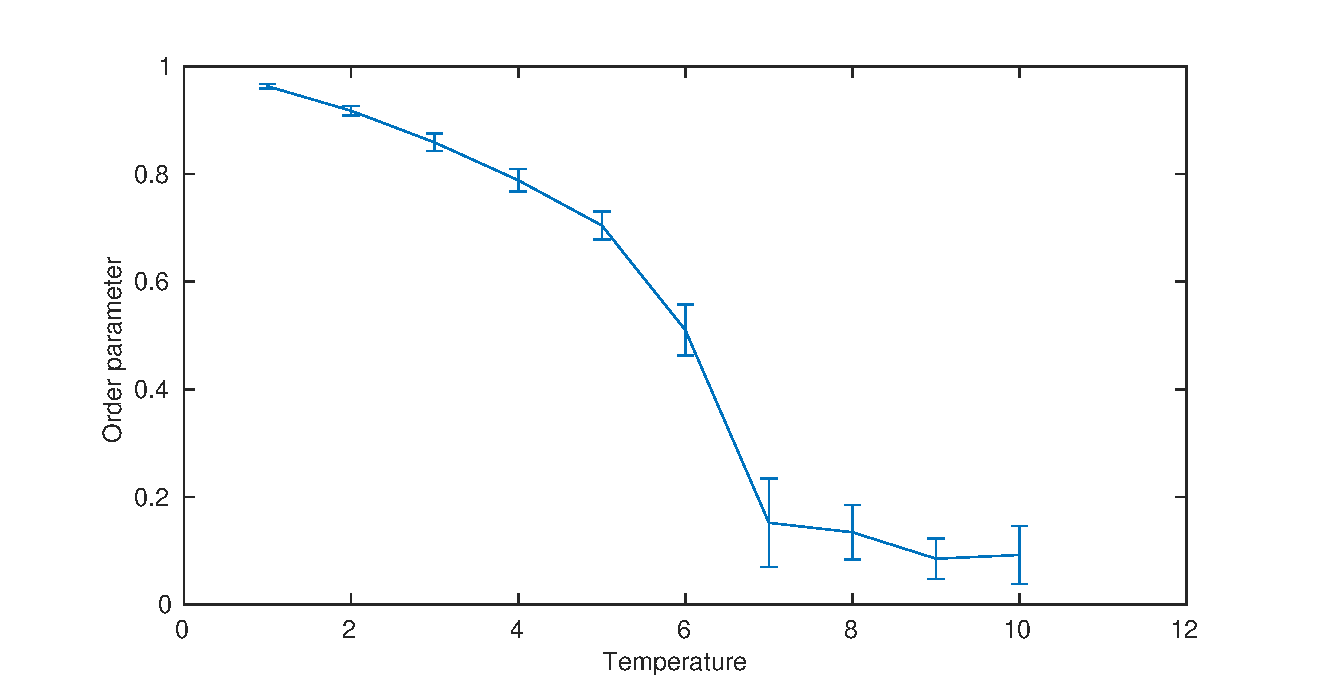
\includegraphics[width=\textwidth]{OrderTemperature}
\end{figure}
As expected, at low temperatures the system is highly ordered. 
At high temperatures the system becomes disordered.
The standard deviation of the order parameter also increases with temperature, as the random configurations at hgiher temperatures will show varying degrees of instantaneous order.

\end{document}